\documentclass[cjk,slidestop,compress,mathserif,blue]{beamer}
%dvipdfm选项是关键,否则编译统统通不过
%beamer的颜色选项定义的是导航条和标题的颜色(即关键词structure的颜色)

%%%%%%%%%%%%%%%%仅限于XeTeX可使用的宏包%%%%%%%%%%%%%%%%%%%%%%%%%%%%
\usepackage{fontspec,xunicode,xltxtra,beamerthemesplit}
%\usepackage{beamerthemesplit}
\usepackage{handoutWithNotes}		%(讲义)在打印PPT的时候会留出给每一页做注释的部分
\usepackage{xeCJK}
\setCJKmainfont[BoldFont=黑体, ItalicFont=楷体, BoldItalicFont=仿宋]{黑体}
%\setsansfont[Mapping=tex-text]{Adobe 黑体 Std}
%如果装了Adobe Acrobat,可在font.conf中配置Adobe字体的路径以使用其中文字体
%也可直接使用系统中的中文字体如SimSun,SimHei,微软雅黑 等
%原来beamer用的字体是sans family;注意Mapping的大小写,不能写错

\usepackage{listings} 
\lstset{language=Matlab}%代码语言使用的是matlab 
\lstset{breaklines}%自动将长的代码行换行排版 
\lstset{extendedchars=false}%解决代码跨页时,章节标\dots

%%%%%%%%   确定标题和导航条结构的框架     %%%%%%%%%%%%
\usepackage{beamerthemeshadow}                       %
%\usepackage{beamerthemeclassic}%导航条色与背景色一致%
%%%%%%%%%%%%%%%%%%%%%%%%%%%%%%%%%%%%%%%%%%%%%%%%%%%%%%
\setbeamerfont{roman title}{size={}}
%\usepackage{CJK} % CJK 中文支持                                  %
\usepackage{amsmath,amsthm,amsfonts,amssymb,bm}
\usepackage{bbding}
\usepackage{mathrsfs}
\usepackage{xcolor}                                        %使用默认允许使用颜色
\usepackage{hyperref} 
\usepackage{graphicx}
\usepackage{subfigure}           %图片跨页
\usepackage{animate}		 %插入动画
\usepackage{caption}
\captionsetup{font=footnotesize}

%\usepackage[version=3]{mhchem}		%化学公式
\usepackage{chemformula}
\usepackage{chemfig}		%化学公式

\usepackage{multirow}
\usepackage{makecell}		%允许单元格内换行

\usepackage[dvipdfmx]{movie15_dvipdfmx} %插入视频
%\usepackage{handoutWithNotes}		%(讲义)在打印PPT的时候会留出给每一页做注释的部分
%\pgfpagesuselayout{1 on 1 with notes landscape}[a4paper,border shrink=5mm]

%\usepackage[numbers,sort&compress]{natbib} %紧密排列             %
\usepackage[sectionbib]{chapterbib}        %每章节单独参考文献   %
\usepackage{hypernat}                                                                         %
\setbeamertemplate{bibliography item}[text] %参考文献前标注[]
%\usepackage[dvipdfm,bookmarksopen=true,pdfstartview=FitH,CJKbookmarks]{hyperref}		%
\hypersetup{bookmarksnumbered,colorlinks,linkcolor=brown,citecolor=blue,urlcolor=red}         %
%参考文献含有超链接引用时需要下列宏包,注意与natbib有冲突        %
%\usepackage[dvipdfm]{hyperref}                                  %
%\usepackage{hypernat}                                           %
\newcommand{\upcite}[1]{\hspace{0ex}\textsuperscript{\cite{#1}}} %
%%%%%%%%%%%%%%%%%%%%%% BIBTEX 引用参考文献 支持\footfullcite{} 引用 %%%%%%%%%%%%%%%%%%%%%%%%%%%%%%%%%%%
%\usepackage{filecontents}%%%%%生成一个main.bib文件
%\begin{filecontents*}{main.bib}
%@BOOK{Xu-Li-II,
%  author = {徐光宪,黎乐民,王德民},
%  title = {{\textit 量子化学——基本原理和从头计算法}{\rm(中)}},
%  publisher = {科学出版社},
%  year = {2001},
%  address = {北京},
%  edition = {1st},
%}
%
%@ARTICLE{PRB136-864_1964,
%  author = {P. Hohenberg and W. Kohn},
%  title = {Inhomogeneous electron gas.},
%  journal = {Phys. Rev.},
%  year = {1964},
%  volume = {136},
%  number = {},
%  pages = {B864},
%  month = {},
%  note = {},
%  otherinfo = {}
%}
%\end{filecontents*} %%%%%生成一个main.bib文件结束
%\usepackage[backend=bibtex,sorting=none]{biblatex}
%%\usepackage[backend=bibtex,style=authoryear]{biblatex}
%\addbibresource{main} %BibTeX数据文件及位置(位置)
%%\addbibresource{Ref_2020-03-04} %BibTeX数据文件及位置(文件)
%%\setbeamerfont{footnote}{size=\tiny} %设置footnote字体
%\setbeamerfont{footnote}{size=\fontsize{5.2pt}{1.9pt}\selectfont}
%%%%%%%%%%%%%%%%%%%%%%BIBTEX 引用参考文献 支持\footfullcite{} 引用%%%%%%%%%%%%%%%%%%%%%%%%%%%%%%%%%%%

%\usepackage{marvosym} %插入各种符号

%\useoutertheme{smoothbars}
\useinnertheme[shadow=true]{rounded}
\usetheme{Berkeley}                                          %主题式样
%\usetheme{Luebeck}

\usecolortheme{lily}                                        %颜色主题式样

\usefonttheme{professionalfonts}                           %字体主题样式宏包

%\beamertemplatetransparentcoveredhigh                      %使所有被隐藏的文本高度透明
\beamertemplatetransparentcovereddynamicmedium             %使所有被隐藏的文本完全透明,动态,动态的范围很小
\mode<presentation>
%\beamersetaveragebackground{gray}                          %设置背景颜色(单一色) 
\beamertemplateshadingbackground{green!10}{red!5}         %设置背景颜色(渐变色)

%i放置单位logo
%\logo{
\includegraphics[width=1.6cm,height=0.35cm]{Figures/BCC_logo-1.png}}	%简单设置logo

%\pgfdeclareimage[width=3.5cm]{logoname}{Figures/BCC_logo-1.png}		%logo置于左侧微调
%\logo{\pgfuseimage{logoname}{\vspace{0.2cm}\hspace*{-2.0cm}}}

%在指定位置精确放置logo
\usepackage{tikz}
\usepackage{beamerfoils}
\usepackage{pgf}
\logo{\pgfputat{\pgfxy(11.68,0.15)}{
\includegraphics[height=1.01cm,viewport=0 0 140 120,clip]{Figures/BCC_logo-1.png}}\pgfputat{\pgfxy(10.502,-0.218)}{
\includegraphics[height=0.369cm,viewport=140 0 540 120,clip]{Figures/BCC_logo-1.png}}}
%\logo{\pgfputat{\pgfxy(11.68,0.15)}{
\includegraphics[height=0.95cm,viewport=0 0 510 360,clip]{Figures/Logo_Gainstrong.png}}\pgfputat{\pgfxy(10.333,-0.195)}{
\includegraphics[height=0.35cm,viewport=530 70 1100 218,clip]{Figures/Logo_Gainstrong.png}}}
%\logo{\pgfputat{\pgfxy(10.28,0.00)}{
\includegraphics[height=0.95cm,viewport=0 0 1100 360,clip]{Figures/Logo_Gainstrong.png}}}
%\logo{\pgfputat{\pgfxy(11.68,0.15)}{
\includegraphics[height=0.95cm,viewport=0 0 510 360,clip]{Figures/Logo_Gainstrong.png}}\pgfputat{\pgfxy(10.333,-0.195)}{
\includegraphics[height=0.35cm,viewport=530 70 1100 218,clip]{Figures/Logo_Gainstrong.png}}}
%\MyLogo{
%	\pgfputat{\pgfxy(-50,-50)}{\pgfbox[right,base]{
\includegraphics[height=1cm]{Figures/BCC_logo-1.png}}}

%logo作为背景放置
%\setbeamertemplate{background}{
%	\pgfputat{\pgfxy(6.5,-0.5)}{\pgfbox[left,top]{\pgfimage[height=1.1cm]{Figures/BCC_logo-1.png}}}}

%\logo{}									%不显示logo

\begin{document}
%\begin{CJK*}{GBK}{song}
%\begin{CJK*}{GBK}{kai}
%beamer下不能用\songyi、\zihao等命令!

%\renewcommand{\figurename}{\tiny\CJKfamily{hei} 图.}
\renewcommand{\figurename}{\tiny{\bf Fig}.}
%\renewcommand{\tablename}{\tiny\CJKfamily{hei} 表.}
\renewcommand{\tablename}{\tiny{\bf Tab}.}
%\renewcommand{\tablename}{\tiny\CJKfamily{hei} 表.}
%\renewcommand{\thesubfigure}{\roman{subfigure}}  %\makeatletter 子图标记罗马字母
\renewcommand{\thesubfigure}{\tiny(\alph{subfigure})}  %\makeatletter 子图标记英文字母
%\renewcommand{\thesubfigure}{}  \makeatletter %子图无标记

\graphicspath{{Figures/}}

%-------------------------------PPT Title-------------------------------------
\title{标题\rm{标题}}
%-----------------------------------------------------------------------------

%----------------------------Author & Date------------------------------------
\author[\textrm{Author}]{作\;\;者\inst{}} %[]{} (optional, use only with lots of authors)
% - Give the names in the same order as the appear in the paper.
% - Use the \inst{?} command only if the authors have different
%   affiliation.
\institute[CTU]{\inst{}%
 \vskip -30pt 作者单位}
\date[\today] % (optional, should be abbreviation of conference name)
{	{\fontsize{6.2pt}{4.2pt}\selectfont{\textcolor{blue}{E-mail:~}\url{XXXXXXXX@yyyy.ac.cn}}}
\vskip 45 pt \textrm{Date:~Mon/Day/Year}
%\vskip 5 pt {\fontsize{8.2pt}{6.2pt}\selectfont{清华大学\;\;物理系}}
}

% - Either use conference name or its abbreviation
% - Not really information to the audience, more for people (including
%   yourself) who are reading the slides online

\subject{}
% This is only inserted into the PDF information catalog. Can be left
% out.
\frame[allowframebreaks]
{
%	\frametitle{\fontsize{9.5pt}{5.2pt}\selectfont{\textcolor{orange}{“高通量并发式材料计算算法与软件”年度检查}}}
\titlepage
}
%-----------------------------------------------------------------------------

%------------------------------------------------------------------------------列出全文 outline ---------------------------------------------------------------------------------
\section*{}
\frame[allowframebreaks]
{
  \frametitle{Outline}
%  \frametitle{\textcolor{mycolor}{\secname}}
  \tableofcontents%[current,currentsection,currentsubsection]
}
%在每个section之前列出全部Outline
%类似的在每个subsection之前列出全部Outline是\AtBeginSubsection[]
\AtBeginSection[]
{
  \frame<handout:0>%[allowframebreaks]%讲义(handout)不显示 <handout:0> 讲义显示 <handout:1> / %beamer不显示 <beamer:0> beamer显示 <beamer:1>	
  {
    \frametitle{Outline}
%全部Outline中,本部分加亮
    \tableofcontents[current,currentsection]
  }
}

%------------------------------------------------------------------------------PPT main Body------------------------------------------------------------------------------------
\small
\section{\rm{section-1}}
\subsection{\rm{subsection}}       %Bookmark
\frame%[allowframebreaks]
{
	\frametitle{插入图片和字体设置}
\begin{figure}[h!]
\centering
%\vspace{-25.5pt}
%\hspace*{-15.5pt}
%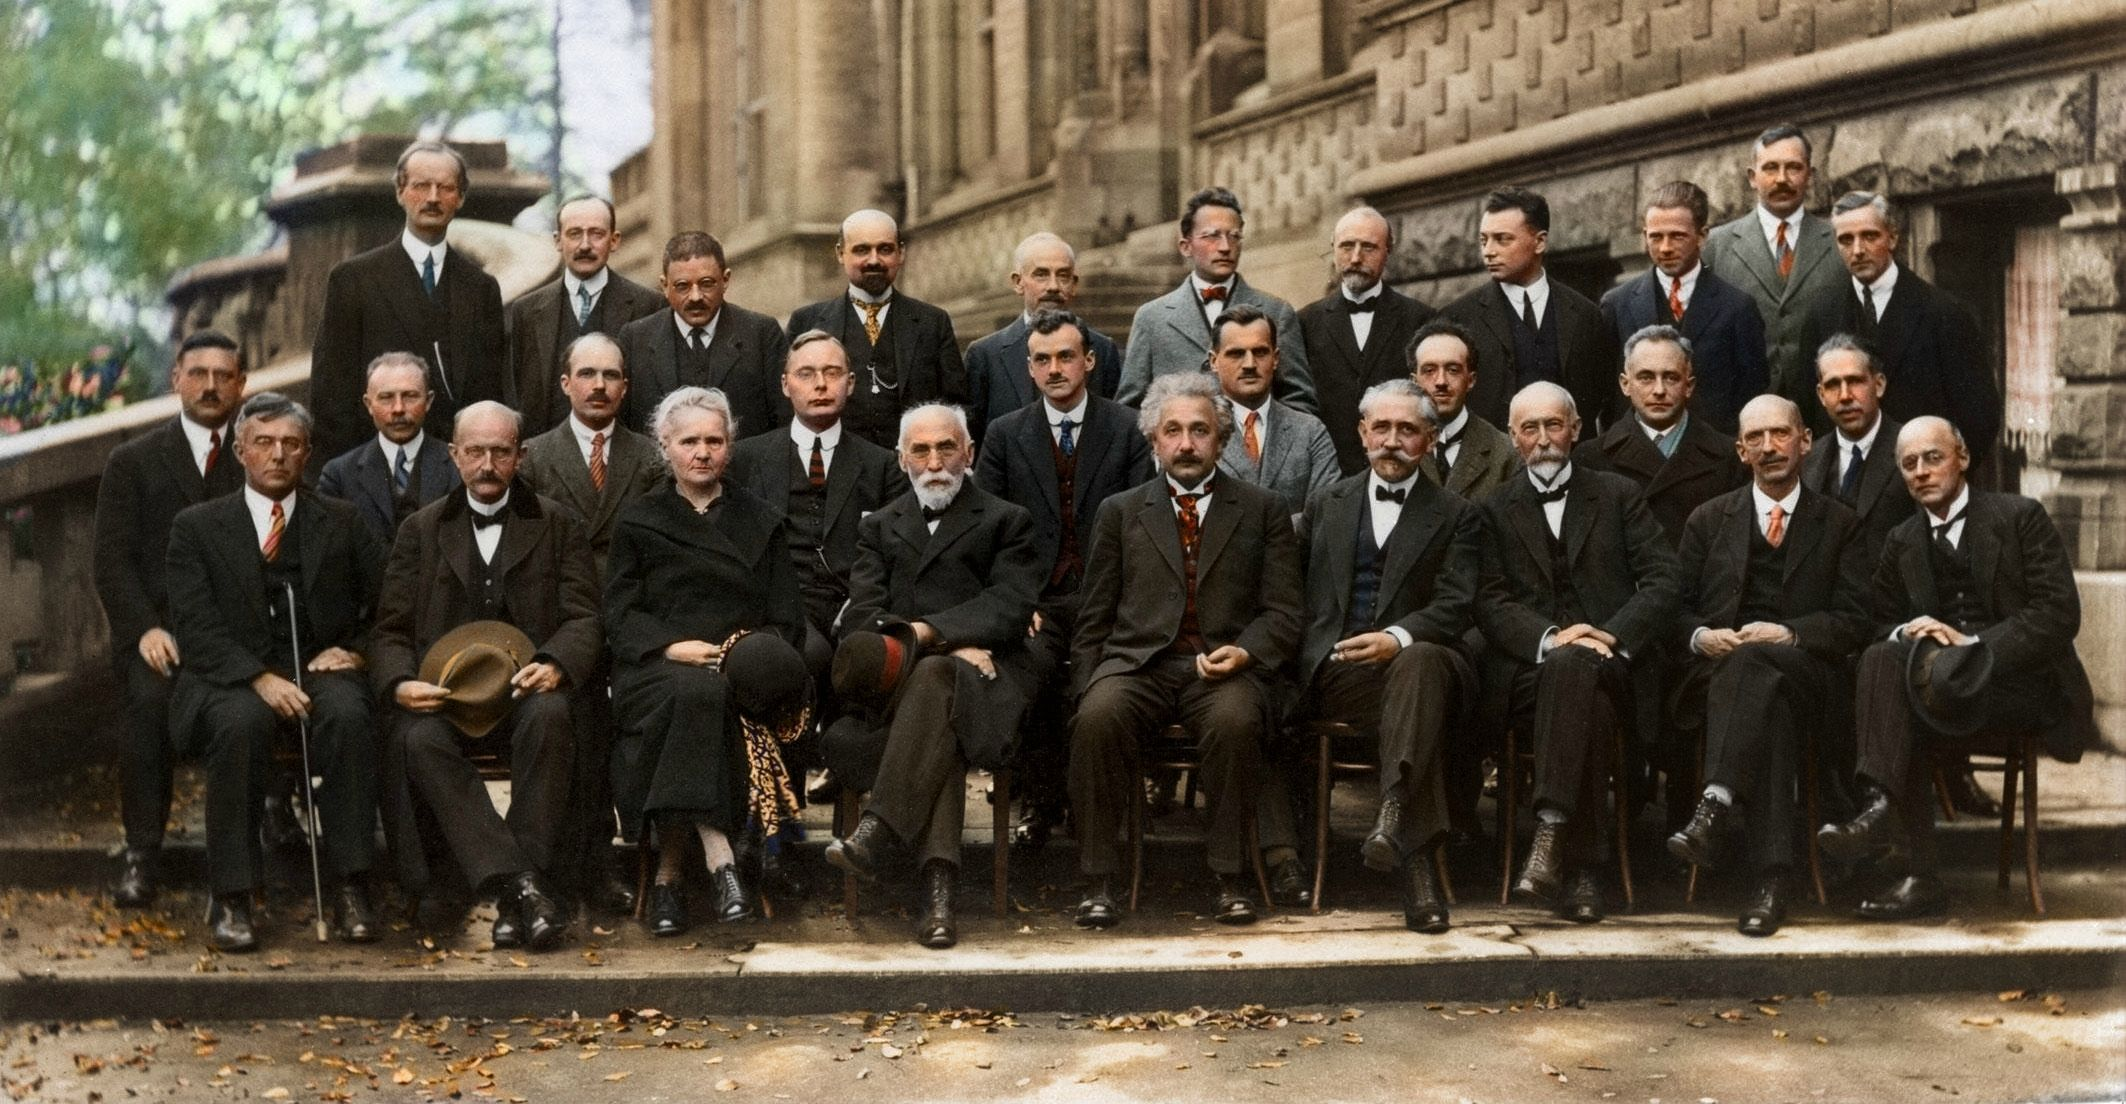
\includegraphics[height=0.57\textwidth,width=1.1\textwidth,viewport=0 0 2150 1050,clip]{Figures/Solvay_Conference-5-fine.jpg}
\vspace{-14.5pt}
\hspace*{-15.5pt}
%\includegraphics[height=0.55\textwidth,width=0.65\textwidth,viewport=150 105 850 710,clip]{Figures/Solvay_Conference-5.jpg}
\includegraphics[height=0.55\textwidth,width=0.65\textwidth,viewport=150 105 850 710,clip]{Solvay_Conference-5.jpg}
\caption{\fontsize{5.5pt}{4.2pt}\selectfont{\textrm{The Fifth Solvay International Conference, Brussels, Belgium, Oct. 1927}}}
\label{Solvay Conference-5-fine}
\end{figure}
\vspace*{-11.5pt}
\fontsize{4.1pt}{3.9pt}\selectfont{\textrm{\textcolor{blue}{前排左起}:~I.Langmuir(\textcolor{blue}{朗缪尔}) M.Planck(\textcolor{blue}{普朗克}) Marie Curie(\textcolor{blue}{居里夫人}) H.Lorentz(\textcolor{blue}{洛仑兹}) A.Einstein(\textcolor{blue}{爱因斯坦}) P.Langevin(\textcolor{blue}{朗之万}) Ch.E.Guye(\textcolor{blue}{古伊}) C.T.R.Wilson(\textcolor{blue}{威尔逊}) O.W.Richardson(\textcolor{blue}{理查森})\\
\textcolor{blue}{中排左起}:~P.Debye(\textcolor{blue}{德拜}) M.Knudsen(\textcolor{blue}{克努森}) W.L.Bragg(\textcolor{blue}{布拉格}) H.A.Kramers(\textcolor{blue}{克莱默}) P.A.M.Dirac(\textcolor{blue}{狄拉克}) A.H.Compton(\textcolor{blue}{康普顿}) L.de Broglie(\textcolor{blue}{德布罗意}) M.Born(\textcolor{blue}{玻恩}) N.Bohr(\textcolor{blue}{玻尔})\\
\textcolor{blue}{后排左起}:~A.Piccard(\textcolor{blue}{皮卡尔德}) E.Henriot(\textcolor{blue}{亨利厄特}) P.Ehrenfest(\textcolor{blue}{埃伦费斯特}) Ed.Herzen(\textcolor{blue}{赫尔岑}) Th.de Donder(\textcolor{blue}{德唐德}) E.Schr\"odinger(\textcolor{blue}{薛定谔}) E.Verschaffelt(\textcolor{blue}{费尔夏费尔特}) W.Pauli(\textcolor{blue}{泡利}) W.Heisenberg(\textcolor{blue}{海森堡}) R.H.Fowler(\textcolor{blue}{富勒}) L.Brillouin(\textcolor{blue}{布里渊})}}
}
%------------------------------------------------------------------------Reference----------------------------------------------------------------------------------------------
\frame[allowframebreaks]
{
	\frametitle{写入数学公式和并排图片}
	\begin{displaymath}
		\rho_{\nu}\mathrm{d}{\nu}=\dfrac{8{\pi}h{\nu}^3}{C^3}\bigg(\dfrac1{\mathrm{e}^{h\nu/kT}-1}\bigg)\mathrm{d}\nu
	\end{displaymath}
\begin{figure}[h!]
\centering
\vspace{-10.5pt}
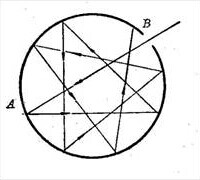
\includegraphics[height=1.45in,width=1.45in,viewport=0 0 136 136,clip]{Black_box.jpg}
\hskip 1pt
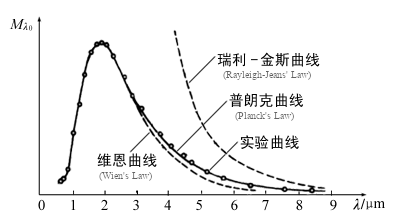
\includegraphics[height=1.32in,width=2.25in,viewport=0 0 390 215,clip]{Black_box_curve.png}
\caption{\tiny\textrm{The black-body radiation and the curve}}
\label{Black_box}
\end{figure}
}

\frame[allowframebreaks]
{
	\frametitle{数学行列式}
	\begin{displaymath}
		\hspace*{-10pt}\Psi(\vec r_1,\vec r_2,\vec r_3,\cdots,\vec r_n)=\dfrac1{\sqrt{n!}}
		\left|\begin{array}{ccccc}
			\psi_1(\vec r_1)&\psi_2(\vec r_1)&\psi_3(\vec r_1)&\cdots&\psi_n(\vec r_1)\\
			\psi_1(\vec r_2)&\psi_2(\vec r_2)&\psi_3(\vec r_2)&\cdots&\psi_n(\vec r_2)\\
			\psi_1(\vec r_3)&\psi_2(\vec r_3)&\psi_3(\vec r_3)&\cdots&\psi_n(\vec r_3)\\
			&&&\cdots&\\
			\psi_1(\vec r_n)&\psi_2(\vec r_n)&\psi_3(\vec r_n)&\cdots&\psi_n(\vec r_n)
		\end{array}\right|
	\end{displaymath}
}

\frame[allowframebreaks]
{
\frametitle{数学矩阵}
	当$|lm^{\prime}\rangle$的基函数是球谐函数,可有
	\begin{displaymath}
		\begin{aligned}
			a_k(m,m^{\prime},m^{\prime\prime},m^{\prime\prime\prime})=&\sum_{q=-k}^k(2l+1)^2(-1)^{m+q+m^{\prime}}\\
			&\times\left(
			\begin{matrix}
				l &k &l\\
				0 &0 &0
			\end{matrix}
			\right)^2\left(
			\begin{matrix}
				l &k &l\\
				-m &q &m^{\prime}
			\end{matrix}\right)\\
			&\times\left(
			\begin{matrix}
				l &k &l\\
				-m^{\prime\prime} &-q &m^{\prime\prime\prime}
			\end{matrix}\right)
		\end{aligned}
	\end{displaymath}
}

\frame[allowframebreaks]
{
	\frametitle{文字以公式的形式对齐和公式中插入文字}
	\begin{displaymath}
%		\hspace*{-2pt}
		\text{电子间瞬时相互作用(\textcolor{red}{关联})}
		\left\{
			\begin{aligned}
				&\text{\textcolor{blue}{电子交换}:同自旋电子的关联作用}\\
				&\text{\textcolor{blue}{电子相关}}
			\end{aligned}
			\right.
	\end{displaymath}
$$\mbox{其中~}D_l(\varepsilon,r)\equiv r\psi_l^{\prime}(r)/\psi_l(r)=r\dfrac{\mathrm{d}}{\mathrm{d}r}\ln\psi_l(r)$$
}

\frame[allowframebreaks]
{
	\frametitle{数学公式换行} 
			\begin{displaymath}
				\begin{aligned}
					E_{\mathrm{TF}}[\rho(\vec r)]=&\dfrac3{10}(3\pi^2)^{\frac23}\int\rho^{\frac53}(\vec r)\mathrm{d}\vec r\\
					&+\int\rho(\vec r)V_{ext}(\vec r)\mathrm{d}\vec r+\dfrac12\int\int\dfrac{\rho(\vec r_1)\rho(\vec r_2)}{|\vec r_2-\vec r_1|}\mathrm{d}\vec r_1\mathrm{d}\vec r_2
				\end{aligned}
			\end{displaymath}
}

\section{\rm{section-2}}
\frame[allowframebreaks]                              %
{
\frametitle{文字图片左右分页}
\begin{minipage}[b]{0.72\linewidth}
 \hspace*{-15pt}
 \begin{itemize}[<+-| alert@+>]
	 \setlength{\itemsep}{10pt}
 \item \textrm{LDA}:泛函只与密度分布的局域值有关
 \item \textrm{GGA}:泛函依赖:局域密度及其梯度
 \item $meta$-\textrm{GGA}:泛函依赖的变量还有动能密度
 \item 杂化(\textrm{hybrid})泛函:泛函与占据轨道有关
 \item 其他的交换-相关能泛函
 \item<1-> 完全非局域泛函:理想泛函,不现实
 \end{itemize}
\end{minipage}
\hfill
\begin{minipage}[b]{0.26\linewidth}
\hspace*{-10pt}
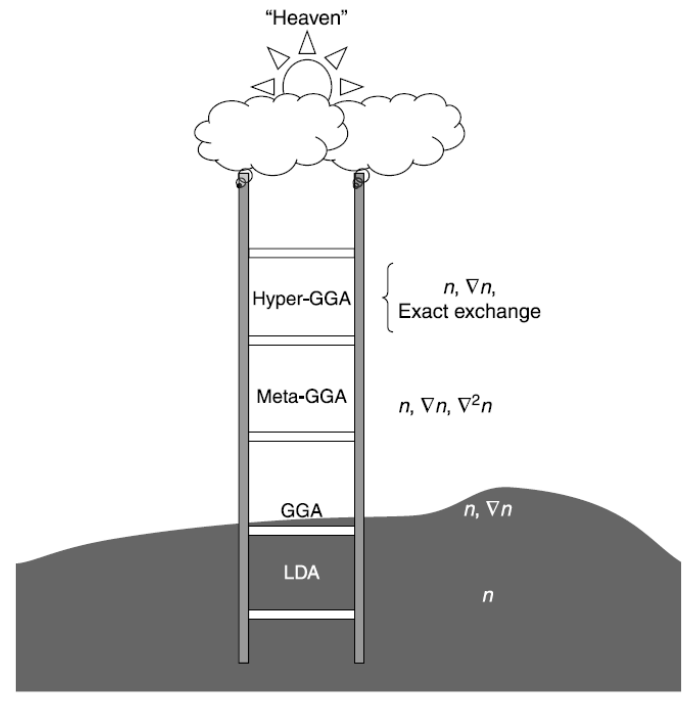
\includegraphics[height=1.7in,width=3.18in,viewport=10 5 1380 700,clip]{Jacobi-ladder.png}\\
{\textcolor{red}{\textrm{Jacob's ladder}}}
\end{minipage}
% \begin{itemize}%[+-| alert@+>]
%\item 交换-相关能密度泛函
}

\frame[allowframebreaks]
{
	\frametitle{列提要(可动态),文字标颜色}
	\begin{itemize}[<+-|alert@+>]
   		%\setlength{\itemsep}{8pt}
		\item<1-2> 波函数假设\\
			\textcolor{blue}{微观体系的运动状态可由波函数$\Psi$完全描述,波函数可以得到体系的所有性质}\\
			波函数$\Psi$一般要求满足\textcolor{red}{连续}、\textcolor{red}{有限}和\textcolor{red}{单值}三个条件
		\item 微观体系的运动状态\textcolor{blue}{波函数随时间变化的规律}:\\\textcolor{red}{遵从\textrm{Schr\"odinger}方程}
			$$\mathrm{i}\hbar\dfrac{\mathrm{d}}{\mathrm{d}t}|\Psi\rangle=\hat{\mathbf H}|\Psi\rangle$$
		\item<3-> 态叠加原理\\
			如果$\Psi_1$是体系的一个本征态,对应的本征值为$A_1$,$\Psi_2$也是体系的一个本征态,对应的本征值为$A_2$,则\textcolor{blue}{$$\Psi=C_1\Psi_1+C_2\Psi_2$$}\textcolor{red}{也是体系一个可能的存在状态}
	\end{itemize}
}

\frame                               %
{
	\frametitle{数字标注提要}
\vskip 20pt
\begin{enumerate}[<+-|alert@+>]
   \setlength{\itemsep}{10pt}
   \item<1-2>  密度是整体变量:~电子自相互作用抵消不净\\%\quad\textrm{(LDA+U)}方法的校正%(\textrm{LDA+U})
	 用\textrm{DFT}计算电子数很少的体系,一般都会有较大的误差
 \item<2->  电子相关:~简并和近简并基态的表示不合理\\
	 基态电子密度用不同的简并轨道计算时,体系能量应保持不变,但现有的近似能量泛函不具有这个性质
 \item<3->  渐近行为:~处理弱相互作用体系的误差大\\
	 如\textrm{Van der Waals}相互作用和现有近似能量泛函本身的计算误差在同一量级
 \end{enumerate}
}

\frame[allowframebreaks]
{
\frametitle{插入子图}
\begin{figure}[h!]
\centering
\hspace*{-0.25in}
\vspace*{-0.1in}
\subfigure[{\tiny 一维$\mathrm{H}$原子链}]{
\label{fig:Hydrogen-1D}
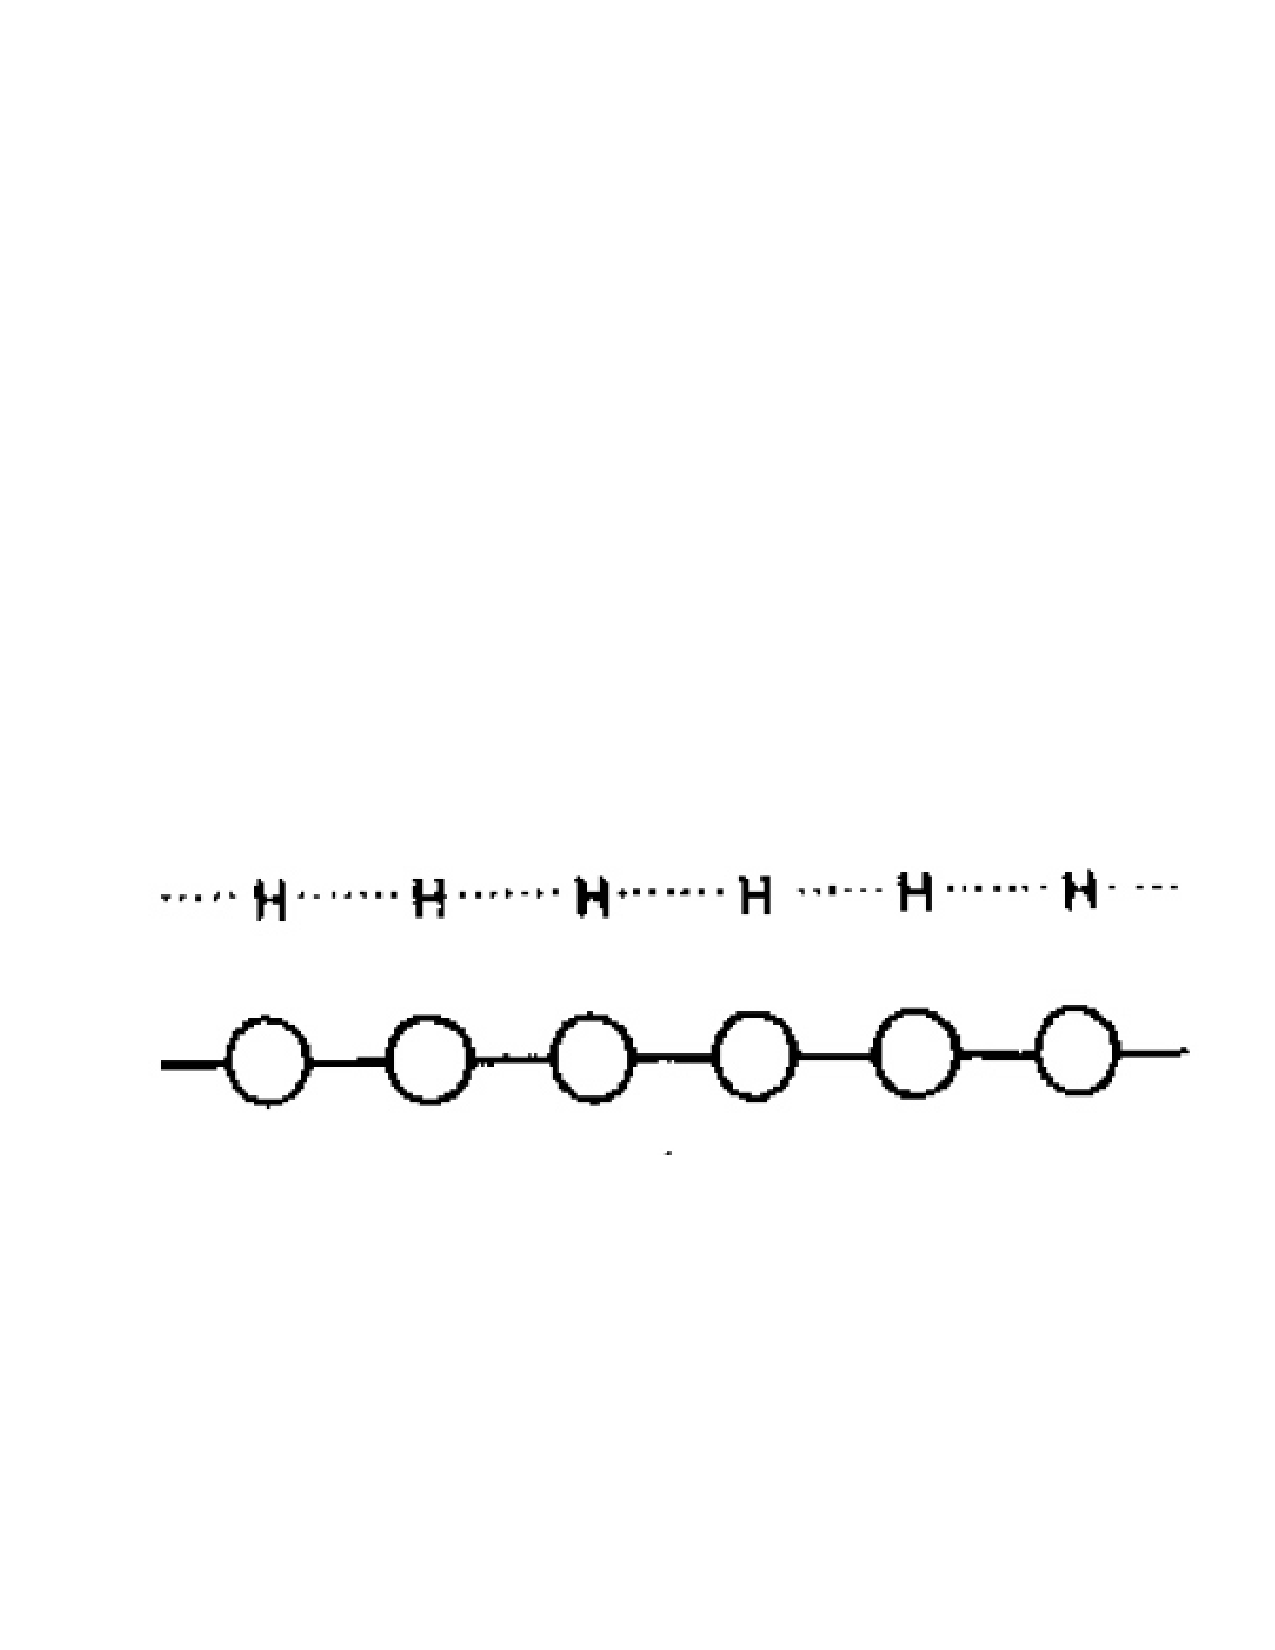
\includegraphics[height=0.25in,width=1.1in,viewport=70 255 570 375,clip]{Hydrogen-1D.pdf}}
\subfigure[{\tiny $\mathrm{H}_n$分子轨道}]{
\label{fig:Hydrogen-2-n}
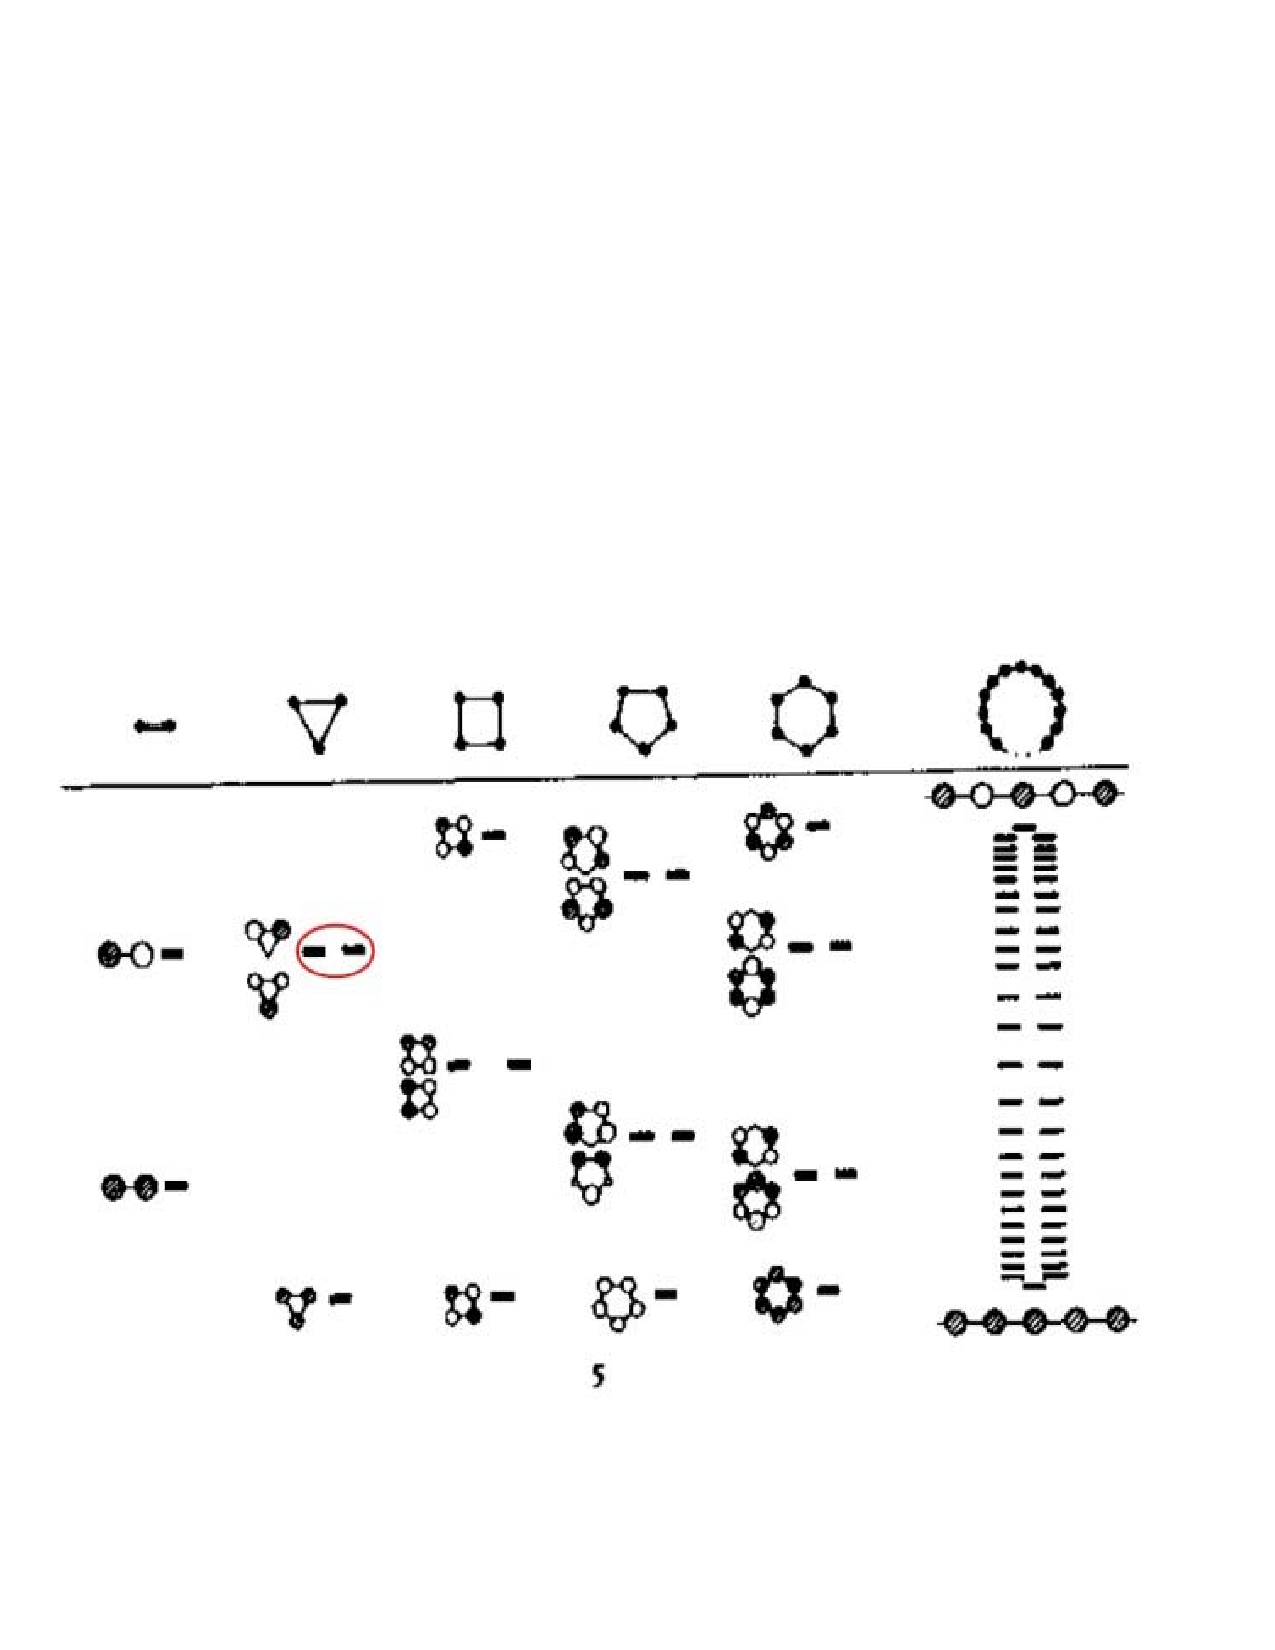
\includegraphics[height=0.8in,width=1.5in,viewport=30 140 545 480,clip]{Hydrogen-Mol-Orbital.pdf}}
\subfigure[{\tiny 分子波函数}]{
\label{fig:Hydrogen-Psi}
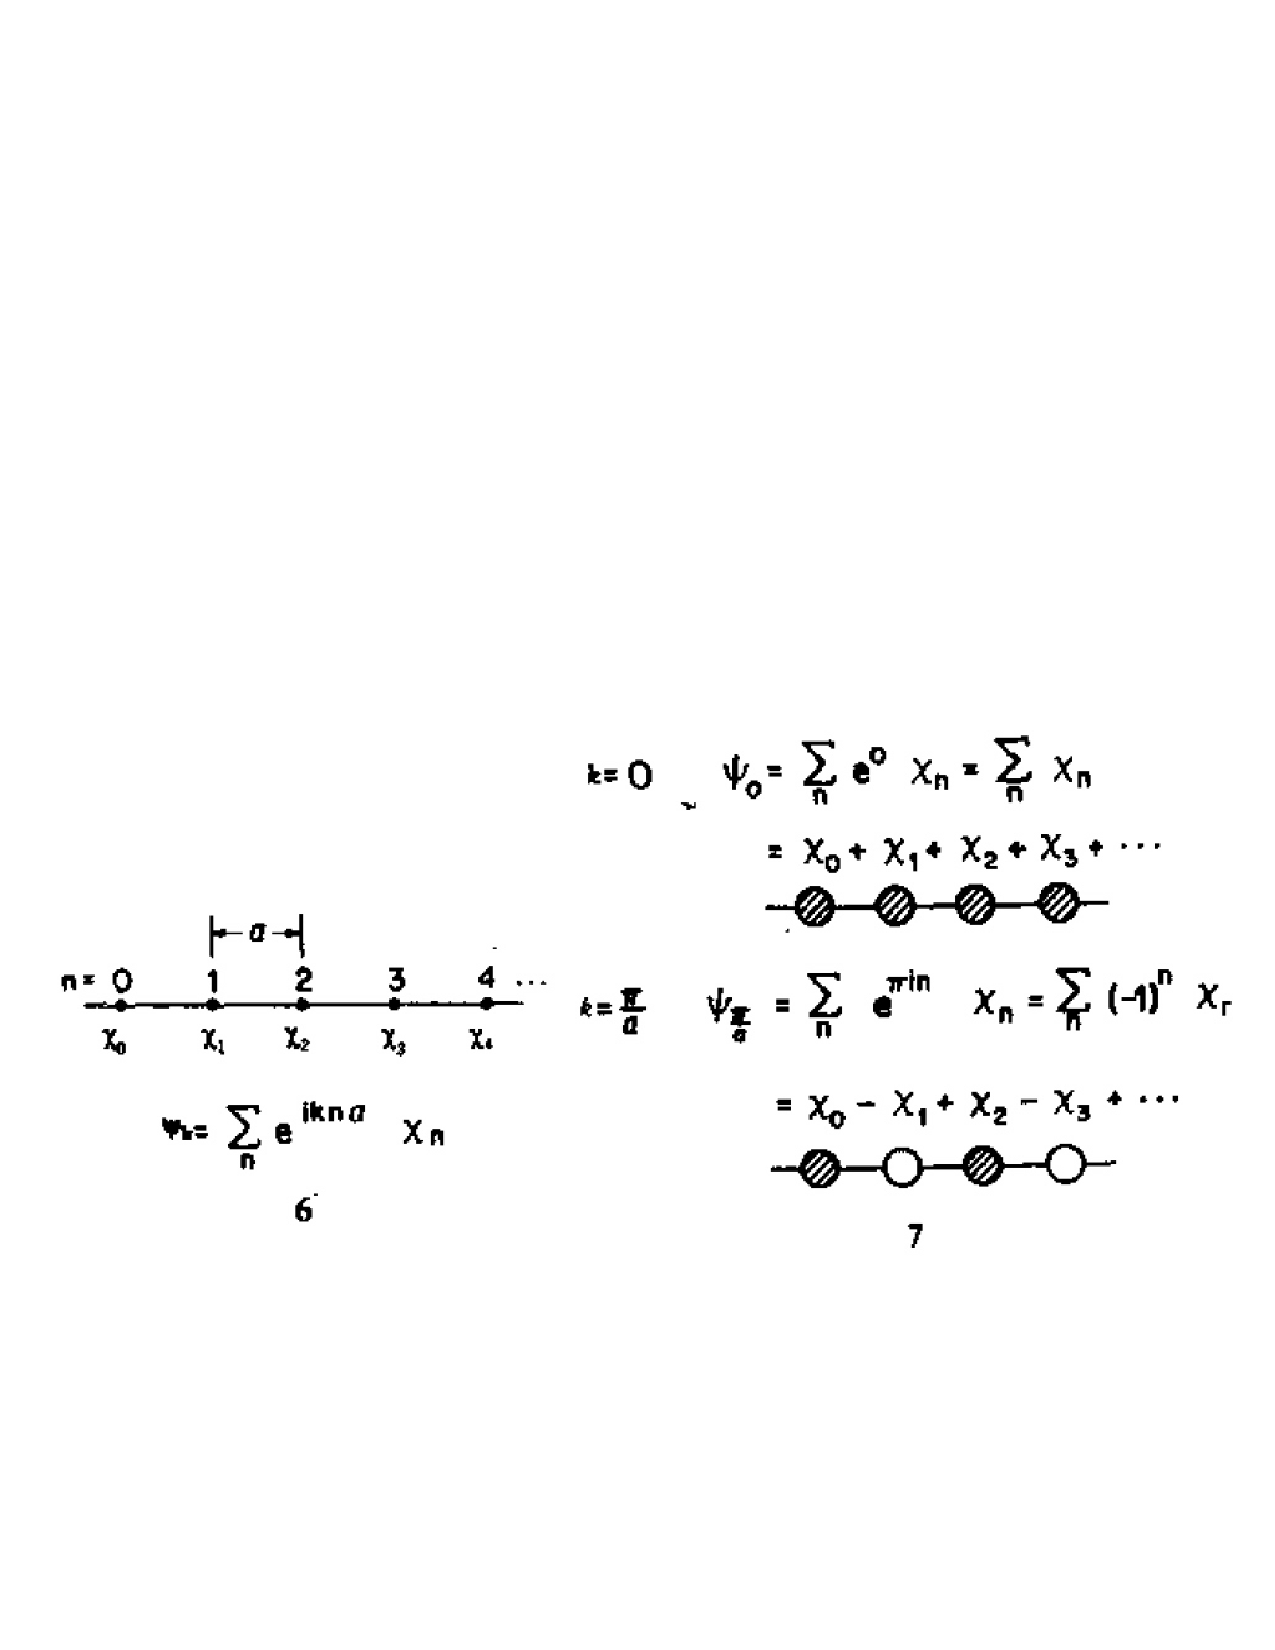
\includegraphics[height=0.5in,width=1.4in,viewport=25 218 595 440,clip]{Hydrogen-Psi.pdf}}\\
\vspace*{5pt}
\subfigure[{\tiny 分子轨道与能带}]{
\label{fig:Hydrogen-Band-1D}
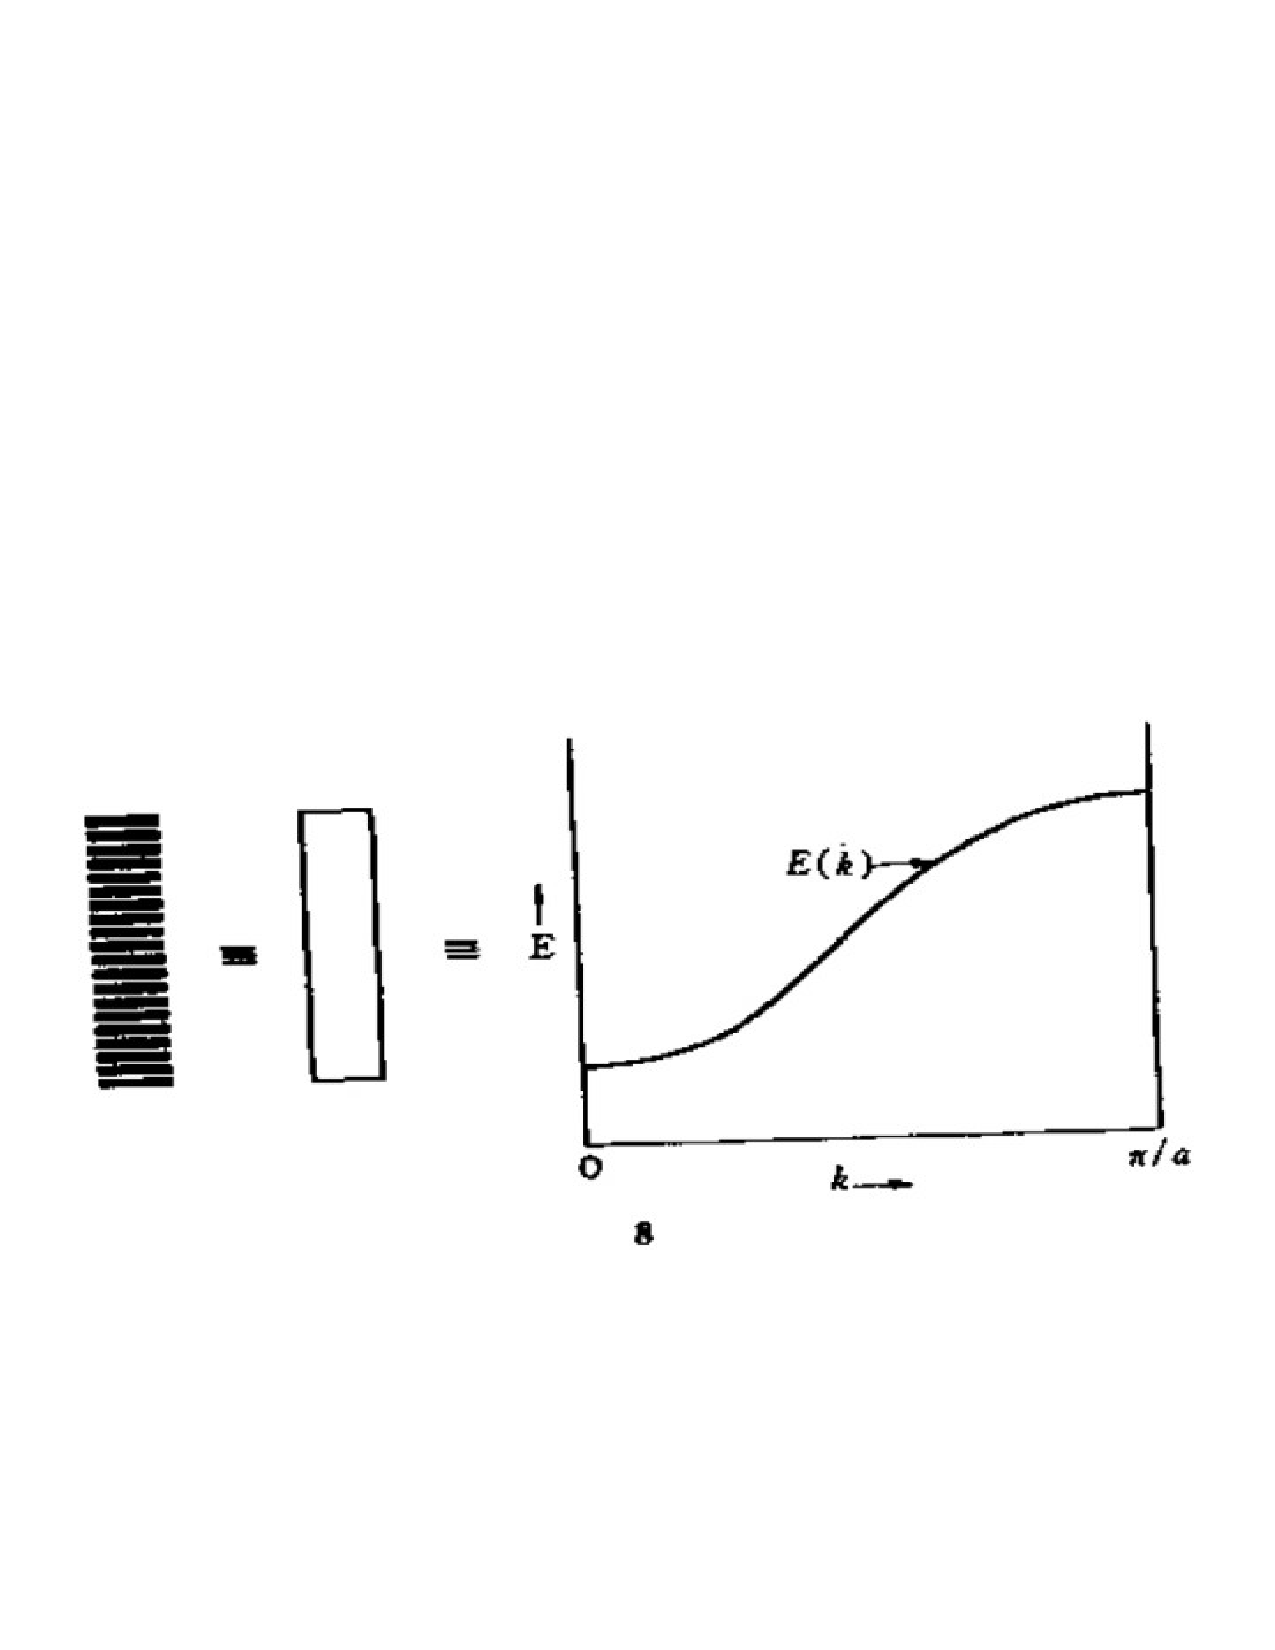
\includegraphics[height=0.6in,width=1.4in,viewport=35 215 575 450,clip]{Hydrogen-Band-1D.pdf}}
\subfigure[{\tiny $d$\,轨道}]{
\label{fig:Hydrogen-d-Band-1D}
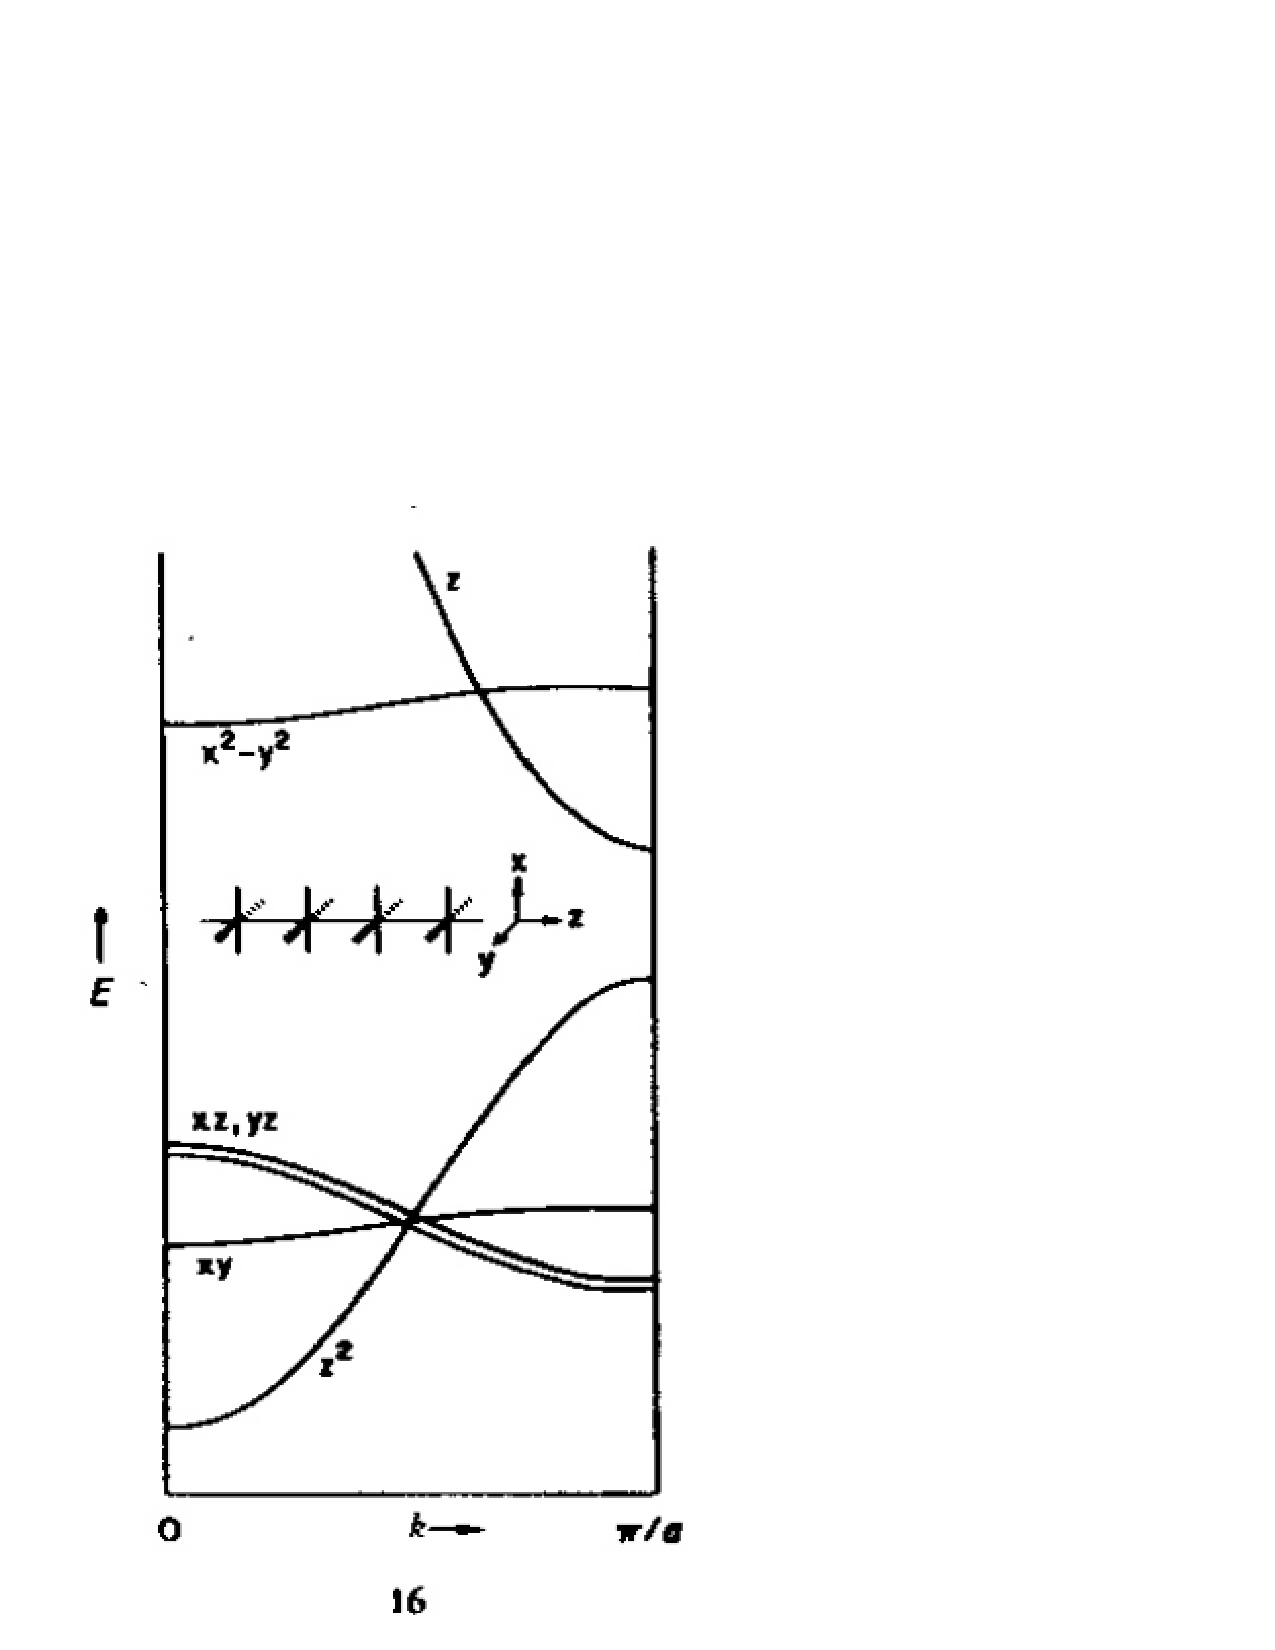
\includegraphics[height=1.0in,width=0.7in,viewport=40 45 330 535,clip]{Hydrogen-d-Band-1D.pdf}}
\caption{\tiny \textrm{The Band-structure from Molecular-orbital.}}%
\label{Band-Structure-local-orbit}
\end{figure} 
}

\frame[allowframebreaks]
{
	\frametitle{表格}
\begin{table}[!h]
\tabcolsep 0pt \vspace*{-5pt}
\caption{\fontsize{8.0pt}{4.2pt}\selectfont{国内外现有自动流程软件概况}}
\label{Table-Cost}
\vskip -12pt
%\begin{center}
\centering
\def\temptablewidth{0.9\textwidth}
\renewcommand\arraystretch{0.8} %表格宽度控制(普通表格宽度的两倍)
\rule{\temptablewidth}{1pt}
%\begin{tabular*} {\temptablewidth}{@{\extracolsep{\fill}}c@{\extracolsep{\fill}}c@{\extracolsep{\fill}}c@{\extracolsep{\fill}}c@{\extracolsep{\fill}}c@{\extracolsep{\fill}}c@{\extracolsep{\fill}}c}
\begin{tabular*} {\temptablewidth}{|@{\extracolsep{\fill}}c|@{\extracolsep{\fill}}c|@{\extracolsep{\fill}}c|@{\extracolsep{\fill}}c|@{\extracolsep{\fill}}c|@{\extracolsep{\fill}}c|@{\extracolsep{\fill}}c|}
%-------------------------------------------------------------------------------------------------------------------------
	&\multirow{2}{*}{\fontsize{5.2pt}{4.2pt}\selectfont{编程语言}}	&\fontsize{5.2pt}{4.2pt}\selectfont{建模~~~~~~} &\multicolumn{2}{c|}{\fontsize{4.2pt}{3.2pt}\selectfont{任务提交与管理}} &\multirow{2}{*}{\fontsize{5.2pt}{4.2pt}\selectfont{后处理~~~~}} &\multirow{2}{*}{\fontsize{4.2pt}{3.2pt}\selectfont{数据组织管理}} \\\cline{4-5}
	&	&\fontsize{5.2pt}{4.2pt}\selectfont{功能~~~~~~} &\fontsize{5.2pt}{4.2pt}\selectfont{软件接口~~~~} &\fontsize{5.2pt}{4.2pt}\selectfont{运行容错~~~~~~~} & & \\\hline
	\fontsize{5.2pt}{4.2pt}\selectfont{{AFLOW}} &\fontsize{5.2pt}{4.2pt}\selectfont{C++} &\checkmark &$\triangle$ &\FiveStarOpen &\FiveStarOpen &\fontsize{5.2pt}{4.2pt}\selectfont{{Django}} \\
	\fontsize{5.2pt}{4.2pt}\selectfont{{MP}} &\fontsize{5.2pt}{4.2pt}\selectfont{Python} &\checkmark &\checkmark &\FiveStarOpen &\FiveStarOpen &\fontsize{5.2pt}{4.2pt}\selectfont{{MongoDB}} \\
	\multirow{2}{*}{\fontsize{5.2pt}{4.2pt}\selectfont{{QMIP}}} &\fontsize{5.2pt}{4.2pt}\selectfont{JavaScript/SVG} &\multirow{2}{*}{\checkmark} &\multirow{2}{*}{\checkmark} &\multirow{2}{*}{--} &\multirow{2}{*}{\checkmark} &\multirow{2}{*}{--} \\
	&\fontsize{5.2pt}{4.2pt}\selectfont{+html/Python} & & & & & \\
	\fontsize{5.2pt}{4.2pt}\selectfont{{CEP}} &\fontsize{5.2pt}{4.2pt}\selectfont{Python} &\checkmark &\checkmark &-- &\checkmark &\fontsize{5.2pt}{4.2pt}\selectfont{{Django/MySQL}} \\
	\fontsize{5.2pt}{4.2pt}\selectfont{{ASE}} &\fontsize{5.2pt}{4.2pt}\selectfont{Python} &\FiveStarOpen &\FiveStarOpen &-- &$\triangle$ &-- \\
	\multirow{2}{*}{\fontsize{5.2pt}{4.2pt}\selectfont{{MatCloud}}} &\fontsize{5.2pt}{4.2pt}\selectfont{JavaScript} &\multirow{2}{*}{\checkmark} &\multirow{2}{*}{$\triangle$} &\multirow{2}{*}{\checkmark} &\multirow{2}{*}{\checkmark} &\multirow{2}{*}{\fontsize{5.2pt}{4.2pt}\selectfont{{MongoDB}}} \\
	&\fontsize{5.2pt}{4.2pt}\selectfont{+.NETCore} & & & & &
\end{tabular*}
\rule{\temptablewidth}{1pt}
%\vskip -15pt
%\end{center}
\end{table}
%\begin{description}
%	\item[\FiveStarOpen]~该功能较突出
%	\item[\checkmark]~该功能基本满足需求
%	\item[\triangle]~该功能存在不足
%\end{description}
\fontsize{6.2pt}{3.2pt}\selectfont{
~~~~~~~~\FiveStarOpen~表示该功能较突出;~\checkmark~表示该功能基本满足需求;~$\triangle$~表示该功能存在不足
}
}

\appendix
%------------------------------------------------------------------------Reference----------------------------------------------------------------------------------------------
%\begin{thebibliography}{99}
%-----------------------------------------------------------------------------------------------------------------------------------------------------------------------%
%\frame[allowframebreaks]
%{
%\frametitle{主要参考文献}
%{\small
%\bibitem{Singh_Book}\textrm{D. J. Singh. \textit{Plane Wave, PseudoPotential and the LAPW method} (Kluwer Academic, Boston,USA, 1994)}					%
%  \nocite{*}																				%
%}
%}
%\end{thebibliography}
		\frame[allowframebreaks]
{
\frametitle{主要参考文献}
\begin{thebibliography}{99}
{\tiny
%	\bibitem{Xu_Li_Wang}徐光宪、黎乐民、王德民, {\textit{量子化学——基本原理和从头计算法}}\;\textrm{({\textit{上、中}})}\:科学出版社, 北京, 1980
	\bibitem{Huang_Han}黄昆\:原著、韩汝琦\:改编, {\textit{固体物理学}}\:高等教育出版社, 北京, 1988
	\bibitem{Xie_Lu}谢希德、陆栋\:主编, {\textit{固体能带理论}}\:复旦大学出版社, 上海, 1998
	\bibitem{JPC12-4409_1979}\textrm{J. Ihm, A. Zunger and L. Cohen, {\textit{J. Phys. C}} \textbf{12} (1979), 4409}
	\bibitem{Elect_Stru}\textrm{Richard. M. Martin. \textit{Electronic Structure: Basic Theory and Practical Methods} (Cambridge University Press, Cambridge, England, 2004)}
	\bibitem{PR57-1169_1940}\textrm{C. Herring. \textit{Phys. Rev.}, \textbf{57} (1940), 1169}
	\bibitem{PR116_1959}\textrm{J. C. Phillips and L. Kleinman. \textit{Phys. Rev.} (1959), 116}
	\bibitem{PRL43-1494_1979}\textrm{D. R. Hamann, M. Schl\"uter and C. Chiang. \textit{Phys. Rev. Lett.} \textbf{43} (1979), 1494}
	\bibitem{PRB50-17953_1994}\textrm{P. E. Bl\"ochl. \textit{Phys. Rev.} B, \textbf{50} (1994), 17953}
	\bibitem{PRB59-1758_1999}\textrm{G. Kresse and D. Joubert \textit{Phys. Rev.} B, \textbf{59} (1999), 1758}
	\bibitem{VASP_UG}\textrm{G. Kresse, M. Marsman, and J. Furthm\"uller. \textit{VASP the GUIDE}. Computational Physics, Faculty of Physics, Universit\"at Wien, Austria (2012) \\\url{http://cms.mpi.univie.ac.at/VASP/}}
	\bibitem{Comp_Method}\textrm{V. V. Nemoshkalenko and V. N. Antonov. \textit{Computational Methods in Solid State Physics} (Gordon and Breach Science Publisher, Amsterdam, The Netherlands, 1998)}
	\bibitem{WIEN2k_UG}\textrm{P. Blaha, K. Schwarz, G. Madsen, D. Kvasnicka and J. Luitz. \textit{User's Guide of WIEN2K, An Augmented Plane Wave Plus Local Orbitals Program for Calculating Crystal Properties}. Vienna University of Technology, Inst. of Physical and Theoretical Chemistry, Vienna, Austria (2012)}
	\bibitem{PRB12-3060_1975}\textrm{O. K. Andersen. \textit{Phys. Rev.} B, \textbf{12} (1971), 3060}
	\bibitem{JMP22-2433_1981}\textrm{M. Weiner. \textit{J. Math. Phys.}, \textbf{22} (1981), 2433}
	\bibitem{PRB26-4571_1982}\textrm{M. Weinert, E. Wimmer and A. J. Freeman. \textit{Phys. Rev.} B, \textbf{26} (1982), 4571}
	\bibitem{SSC114-15_2000}\textrm{E. Sj\"ostedt, L. Nordstr\"om and D. J. Singh. \textit{Solid State Commun.}, \textbf{114} (2000), 15}
	\bibitem{PR94-1111_1954}\textrm{W. Kohn and N. Rostocker. \textit{Phys. Rev.} \textbf{94} (1954), 1111}
	\bibitem{Andersen_Book}\textrm{O. K. Andersen. \textit{Computational Methods in Band Theory} (Plenum, New York, USA, 1971)}
	\bibitem{LMTO_Book}\textrm{H. Skriver. \textit{The LMTO method} (Springer, New York, USA, 1984)}
	\bibitem{Crelle30-51_1846}\textrm{C. G. Jacobi,\textbf{\"Uber ein leichtes Verfahren die in der Theorie der S\"acul\"arst\"orrungen vorkommenden Gleichungen numerisch aufzul\"osen}, \textit{Crelle's J.} \textbf{30} (1846), 51-94}
        \bibitem{CMS6-15_1996}\textrm{G. Kresse and J. Furthm\"uller \textit{Comput. Mat. Sci.}, \textbf{6} (1996), 15}
	\bibitem{PRB54-11169_1996}\textrm{G. Kresse and J. Furthm\"uller \textit{Phys. Rev.} B, \textbf{54} (1996), 11169}
	\bibitem{PRB7-5212_1973}\textrm{A. Baldereschi \textit{Phys. Rev.} B, \textbf{7} (1973), 5212}
	\bibitem{PRB8-5747_1973}\textrm{D. J. Chadi and M. L. Cohen \textit{Phys. Rev.} B, \textbf{8} (1973), 5747}
	\bibitem{PRB13-5188_1976}\textrm{H. J. Monkhorst and J. D. Pack \textit{Phys. Rev.} B, \textbf{13} (1976), 5188}
	\bibitem{PA13-392_1947}\textrm{J. Korringa. \textit{Physica}, \textbf{13} (1947), 392}
	\bibitem{JPCM14-2799_2002}\textrm{N. Papanikolaou, R. Zeller and P. H. Dederichs. \textit{J. Phys.: Condens. Matter.} \textbf{14} (2002), 2799}
	\bibitem{PRB44-943_1991}\textrm{V. I. Anisimov, J. Zaanen and O.K. Andersen. \textit{Phys. Rev.} B, \textbf{44} (1991), 943}
	\bibitem{PRB48-16929_1993}\textrm{V.I. Anisimov, I.V. Solovyev, M.A. Korotin, M.T. Czyzyk and G.A. Sawatzky. \textit{Phys. Rev.} B, \textbf{48} (1993), 16929}
	\bibitem{Dai_Qian}戴道生,钱昆明, {\textit{铁磁学}}(上册),\:科学出版社, 北京, 1998
	\bibitem{JPCSSP13-2675_1980}\textrm{A. H. MacDonald, W. E. Pickett and D. D. Koelling. \textit{J. Phys. C: Solid St. Phys.}, \textbf{13} (1980), 2675}
	\bibitem{PRB62-11556_2000}\textrm{D. Hobbs, G. Kresse and J. Hafner. \textit{Phys. Rev.} B, \textbf{62} (2000), 11556}
}
\end{thebibliography}
\nocite*{}
}

%-----------------------------------------------------------Beamer下使用bib,注意文献罗列--------------------------------------------------------------------------%
\frame[allowframebreaks]
{
\frametitle{主要参考文献}
{\tiny\textrm{
%%\phantomsection\addcontentsline{toc}{section}{Bibliography}	 %直接调用\addcontentsline命令可能导致超链指向不准确,一般需要在之前调用一次\phantomsection命令加以修正	%
%%\phantomsection\addcontentsline{toc}{section}{主要参考文献}	 %直接调用\addcontentsline命令可能导致超链指向不准确,一般需要在之前调用一次\phantomsection命令加以修正	%
\bibliography{Ref_2020-Template}%
\bibliographystyle{../ref/mybib}%
%\bibliographystyle{../Reference/mybib}%
}}
\nocite{*}
}
%------------------------------------------------------------------------------------------------------------------------------------------------------------------------------%

%-------------------------------------------------------------------------------------------------------------------------------------------------------------------------------
\section{附录与几种文献引用方式}
\frame[allowframebreaks]
{
	\frametitle{几种文献引用的方式}
	文献引用\upcite{Huang_Han,Xie_Lu,Xu-Li-I-II,Dai_Qian,Many-Body_Theory,JPC-SSP12-4409_1979,WIEN2K-UG_2001,VASP_manual,PCCP8-3172_2006,Xu_Li_Wang}

	\textcolor{magenta}{\textrm{Beamer}要使用当页脚注引用参考文献,须使用\textrm{biblatex}包,并用\textbackslash\!footfullcite\{label\}引用\\
	\textcolor{red}{注意:~}\textrm{biblatex}与\textrm{chapterbib}不兼容}
\begin{thebibliography}{99}
	\fontsize{5.2pt}{1.9pt}\selectfont{
	\bibitem{Xu_Li_Wang}徐光宪、黎乐民、王德民, {\textit{量子化学——基本原理和从头计算法}}\;\textrm{({\textit{上、中}})}\:科学出版社, 北京, 1980}
\end{thebibliography}
\nocite*{}
}

%------------------------------------------------------------------------Reference----------------------------------------------------------------------------------------------
%\begin{thebibliography}{99}
%-----------------------------------------------------------------------------------------------------------------------------------------------------------------------%
%\frame[allowframebreaks]
%{
%\frametitle{主要参考文献}
%{\small
%\bibitem{Singh_Book}\textrm{D. J. Singh. \textit{Plane Wave, PseudoPotential and the LAPW method} (Kluwer Academic, Boston,USA, 1994)}					%
%  \nocite{*}																				%
%}
%}
%\end{thebibliography}

%-----------------------------------------------------------Beamer下不建议使用bib,因为涉及分页--------------------------------------------------------------------------%
%\frame[allowframebreaks]
%{
%\frametitle{主要参考文献}
%{\tiny\textrm{
%%\phantomsection\addcontentsline{toc}{section}{Bibliography}	 %直接调用\addcontentsline命令可能导致超链指向不准确,一般需要在之前调用一次\phantomsection命令加以修正	%
%%\phantomsection\addcontentsline{toc}{section}{主要参考文献}	 %直接调用\addcontentsline命令可能导致超链指向不准确,一般需要在之前调用一次\phantomsection命令加以修正	%
%\bibliography{../ref/Myref}																			%
%\bibliographystyle{../ref/mybib}																		%
%}}
%\nocite{*}																				%
%}
%------------------------------------------------------------------------------------------------------------------------------------------------------------------------------%

%-------------------------------------------------------------------------Thanks------------------------------------------------------------------------------------------------
%\section{致谢}
%\frame[allowframebreaks]
%{
%\frametitle{致$\quad$谢}
%\begin{itemize}
%    \setlength{\itemsep}{20pt}
%  \item 感谢本团队高兴誉、吴泉生、宋红州等各位老师参与的讨论
%  \item 感谢莫所长、宋主任以及软件中心各位老师和同事
%  \item 感谢王崇愚先生的帮助
%\end{itemize}
%}

\logo{}									%不显示logo
\frame[allowframebreaks]
{
\vskip 60 pt
%\hskip 10pt \textcolor{blue}{\Huge 感谢答辩委员会各位老师\,\textrm{!}}\\
\vskip 35 pt
\hskip 60pt \textcolor{blue}{\Huge 谢谢大家\:!}
%\vskip 15 pt
%\hskip 40pt \textcolor{blue}{\Huge \textrm{for your attention\:!}}
}

%\frame[allowframebreaks]
%{
%\begin{figure}[h!]
%\centering
%\animategraphics[autoplay, loop, height=2.1in]{1}{Figures/Prof_Liu-}{06}{11}
%\label{Prof_Liu}
%\end{figure}
%}
%
%-------------------------------------------------------------------------------------------------------------------------------------------------------------------------------
%\paragraph{}
\clearpage
%\end{CJK*}
\end{document}
